\section{Introduction}

The Gut-microbiome is by far the best and widely studied microbial ecosystem of the human anatomy, partly due to the rich microbial environment and partly due to the ease of sample collection (non-invasive) through faeces \cite{Budden2017}. On the other hand, healthy lung was long considered to be sterile but with advent high-throughput sequencing techniques this has been proven otherwise [cite]. Extensive research on the gut-microbiota has that shown that gut microbiota is capable of influencing other organs, such as the brain, liver or lungs \cite{Bell2019}. This has led to the coining of terms such as the `gut–brain axis' and the `lung-gut axis'. 

The epithelial surfaces of the gut and lung are exposed to diverse microbes; ingested microorganisms can access both sites and the microbiota from the gut can enter the lungs through processes such as micro-aspiration \cite{Budden2017}. Furthermore, the lung and gut can interact thorough the systemic cytokines released by host immune cells in response to microbes or  microbes from one-site may secrete metabolites which are absorbed into the blood stream and thus regulate the organs \cite{Dang2019}. A study used germ free mice, which lack an appropriately developed immune system and showed mucosal alterations, both of which is restored through colonization with gut microbiota. Thus, supplementing the concept of `lung-gut' axis \cite{Budden2017}. 

Literature survey using the keyword `lung-gut axis' shows that this concept was first introduced in 2004 and increasing work is being done \ref{ch2_fig1}. This increasing evidence also suggests, a potential existence of lung-gut axis and its effectual role in lung diseases. Although the gut–lung axis is only beginning to be understood, emerging evidence indicates that there is potential for manipulation of the gut microbiota in the treatment of lung diseases. Despite this, the influence of microbial gut health in Bronchiectasis lung is poorly studied. Hence, in the second chapter of my PhD thesis

\begin{figure}[ht]
	\centering
	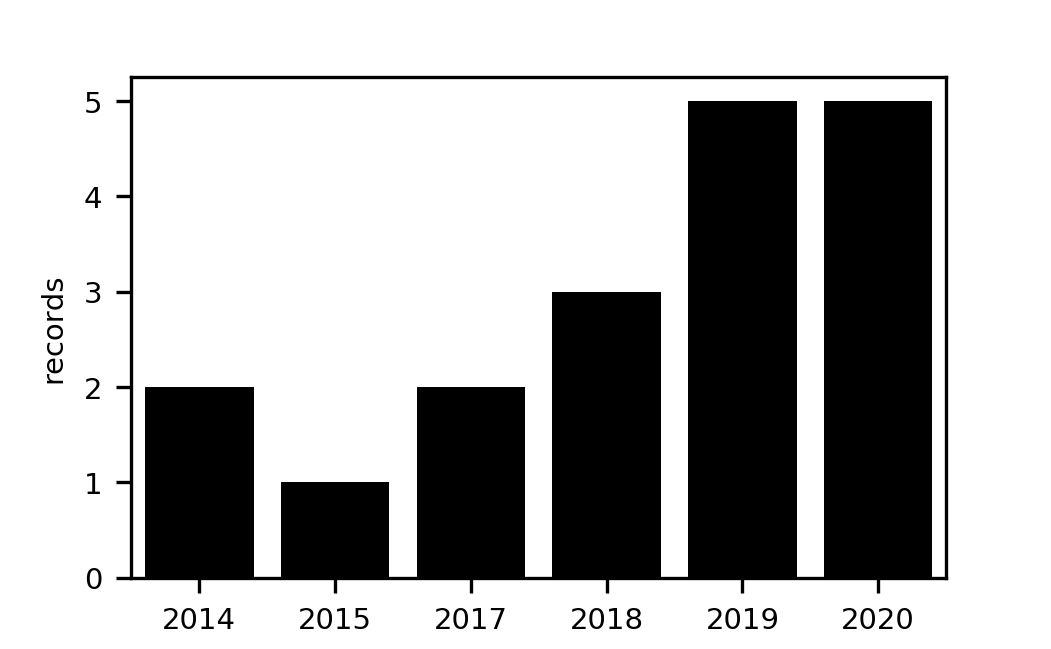
\includegraphics[width=0.5\textwidth]{./image/bar-papers.png}
	\caption{A histogram illustrating all available publications (including original articles and perspectives) matching the keyword ``lung-gut axis" from 1900 to 2020 in the web of science database.}
	\label{ch2_fig1}
\end{figure}
		









 



Want to check if microbes interact